\documentclass[12pt]{article}

\usepackage{sbc-template}
\usepackage{graphicx,url}
\usepackage[utf8]{inputenc}
\usepackage[brazil]{babel}
\usepackage[latin1]{inputenc}  
\usepackage{amsmath}


\sloppy

\title{Instructions for Authors of SBC Conferences\\ Papers and Abstracts}

\author{Luciana P. Nedel\inst{1}, Rafael H. Bordini\inst{2}, Flávio Rech
  Wagner\inst{1}, Jomi F. Hübner\inst{3} }


\address{Instituto de Informática -- Universidade Federal do Rio Grande do Sul
  (UFRGS)\\
  Caixa Postal 15.064 -- 91.501-970 -- Porto Alegre -- RS -- Brazil
\nextinstitute
  Department of Computer Science -- University of Durham\\
  Durham, U.K.
\nextinstitute
  Departamento de Sistemas e Computação\\
  Universidade Regional de Blumenal (FURB) -- Blumenau, SC -- Brazil
  \email{\{nedel,flavio\}@inf.ufrgs.br, R.Bordini@durham.ac.uk,
  jomi@inf.furb.br}
}

\begin{document} 

\maketitle

\begin{abstract}
Video streaming services have been experiencing changes in the recent years, where the number of users consuming a variety of video streaming has been increasing exponentially in Live and Video-on-Demand~(VoD) platforms. In order to accommodate the growing video traffic demand, new solutions have to be designed for the Future of the Internet to provide good users' Quality of Experience~(QoE). This work focus on code a Resource Assignment mechanism capable to provide a video streaming service inside a multi-tier edge/cloud architecture. In this way, this research work also evaluate the impact on the performance of VoD introduced by new distributed computing infrastructures in edge/cloud computing scenarios.
\end{abstract}
     
\begin{resumo} 
Os serviços de streaming de vídeo têm passado por mudanças nos últimos anos, onde o número de usuários consumindo uma variedade de streaming de vídeo tem aumentado exponencialmente nas plataformas Live e Video-on-Demand~(VoD). A fim de acomodar a crescente demanda de tráfego de vídeo, novas soluções devem ser projetadas para o Futuro da Internet para fornecer uma boa qualidade de experiência aos usuários~(QoE). Este trabalho tem como foco codificar um mecanismo de Atribuição de Recursos capaz de fornecer um serviço de streaming de vídeo dentro de uma arquitetura de borda/nuvem multicamadas. Desta forma, este trabalho de pesquisa também avalia o impacto no desempenho do VoD introduzido por novas infraestruturas de computação distribuída em cenários de computação de borda/nuvem.
\end{resumo}



\section{Introduction}
\label{sec:intro}

%******* Introduction of the Dash technology and Cloud/Fog networks****
Atualmente, os conteúdos multimídia são fornecidos a uma infinidade de dispositivos, onde a exigência pela qualidade de imagem muda de acordo com a dispositivos, que vão de pequenos telefones celulares a TVs de alta resolução. Para lidar com uma transmissão de video com diferentes e rigorosos requisitos, como um canal de comunicação de boa qualidade bem como um fluxo constante e ininterrupto de informações~\cite{Immich2018WinNet}. Essa demanda deve manter uma boa Qualidade de Experiencia~(\textit{Quality of Experience} - QoE) do usuário. Hoje, o tráfego multimídia corresponde à maior parte dos dados que circulam pela Internet em todo o mundo, e tal previsão de crescimento se mantém  para os próximos anos. 
Dentro desta rede o protocolo utilizado pelos grandes players do mercado (como Microsoft, Apple, Adobe e Netflix) adotam o paradigma Transmissão Adaptativa HTTP~(\textit{HTTP Adaptive Streaming} - HAS)~\cite{company:dashs}. Hoje, eles são decompostos essencialmente em Servidores HTTP para atender essa demanda.

o cliente e o servidor utilizam o protocolo HTTP na camada de aplicação para realizar todas as requisições/respostas necessárias. No lado do servidor, uma vez que um arquivo de mídia~(ou fluxo) esteja pronto, ele será preparado para streaming antes de ser publicado em um servidor HTTP padrão. O arquivo/stream original é particionado em segmentos~(também chamados \textit{chunks}) de tempo de reprodução equivalente, e várias versões (também chamadas de representações) de cada segmento são geradas que variam em taxa de bits/resolução/qualidade usando um codificador ou um transcodificador.
A lista as representações disponíveis incluem informações como tempo de vídeo, disponibilidade de conteúdo, tipos de mídia~(ou seja, H.264 , H.265, etc. .), resoluções, larguras de banda mínimas e máximas, e a existência de várias alternativas codificadas de componentes multimídia, localização de segmentos de mídia na rede e outras características de conteúdo.

No lado do cliente HAS, o player solicita os segmentos de video sequencialmente e adapta-se dinamicamente às condições da rede usando sua lógica adaptativa de taxa de bits~(ABR). Os esquemas ABR também levam em consideração o buffer de reprodução, recursos do dispositivo, preferências do visualizador, bem como recursos de conteúdo, com pesos diferentes.
Como a QoE do espectador precisa ser determinada em tempo real durante a reprodução, métricas objetivas são frequentemente usadas, incluindo o número de interrupções, duração do atraso de inicialização, frequência e número de oscilações de qualidade de vídeo. Por padrão, o HAS não requer nenhum esquema de adaptação específico, deixando os desenvolvedores de sistemas inovarem e implementarem seus próprios métodos.

% ----------------------------------------------------------------------------
% What is the current context in edge-cloud network in terms of traffic and users? 
% ----------------------------------------------------------------------------
Hoje, as soluções existentes para serviços de streaming de vídeo são projetadas para fornecer conteúdo multimídia em data centers de edge-cloud. Esses sistemas de adaptação baseados em DASH normalmente são capazes de se adequar às condições de entrega de rede tanto na borda quanto na nuvem, o que traz recursos de computação para a borda da rede e, portanto, mais perto dos usuários~\cite{sitaraman:ACD2014}. Dessa forma, a criação desses sistemas resolve parcialmente os problemas de escalabilidade, disponibilidade e interoperabilidade, mas ao mesmo tempo apresenta novos desafios~(por exemplo, maior latência e congestionamento da rede principal)~\cite{tran:wons17,ye: ITC17, taleb:JSAC18}. Vários trabalhos na literatura destacam o fog/edge computing para lidar com as novas demandas de tráfego de vídeo que estão surgindo. Onde data centers com menos capacidade de processamento e armazenamento podem fornecer serviços/virtualização mais próximos do usuário final. Assim, a borda da rede pode fornecer taxas de latência que a nuvem não conseguiria de outra forma~\cite{gamaUCC2019, rosarioSENSORS2018}.

% ----------------------------------------------------------------------------
% What carries have been doing to address the increasing traffic?
% ----------------------------------------------------------------------------

Infelizmente, o uso do MEC aproxima o conteúdo dos usuários móveis, mas também introduz o problema da seleção do MEC. O MEC de serviço pode não ser aquele implantado na BS de serviço. O handover fará com que o usuário se comunique com uma BS alvo, mas não trará a conexão para um MEC vizinho. Portanto, os provedores de conteúdo ou operadoras de rede precisam encontrar um MEC apropriado para cada usuário móvel. Existe a necessidade de um processo de seleção do MEC que deve ser realizado em tempo hábil, a fim de apoiar a alta qualidade do serviço. Um mecanismo de migração de conteúdo na borda e nas camadas superiores pode atenuar o problema. Além disso, realizar um reencaminhamento entre as conexões dos usuários ativos e os nós do servidor pode ajudar a melhorar e equilibrar a QoE do usuário.


Embora muitos trabalhos de pesquisa abordem serviços de streaming de vídeo em conjunto com \textit{fog/cloud computing}, existem aspectos pouco abordados nas soluções atuais~\cite{Mouradian2018ComSurv, bentaeb:2018:MSys}. Geralmente, as arquiteturas de streaming de vídeo buscam diminuir a carga de tráfego e melhorar a QoE da entrega de vídeo. Tais soluções não levam em consideração o comportamento do player de vídeo utilizado pelo usuário, bem como aspectos relacionados à mobilidade do usuário nos mecanismos de tomada de decisão em ambientes multiníveis. A fim de abordar as questões acima, este trabalho tem como objetivo modelar mecanismos de entrega de vídeo em DASH para serem utilizados em ambientes de Smart City. Tais mecanismos propostos aproveitarão tecnologias emergentes relacionadas a redes~ (como computação de borda/nuvem e microsserviços), com o objetivo de auxiliar a tomada de decisão do serviço de streaming de vídeo em uma infraestrutura urbana.

\section{Trabalhos relacionados}
% A multi-tier fog content orchestrator mechanism with quality of experience support

Nesta seção, apresentamos uma comparação entre os trabalhos relacionados sobre video streaming na borda.
De forma geral, as abordagens mencionadas caracterizam-se por diminuir a carga de tráfego e melhorar a QoE.
No entanto, existem armadilhas devido ao comportamento egoista totalmente isolado (ou seja, essas soluções estão funcionando independentemente, sem coordenação) dos players HAS. Os trabalhos de streaming de video abordam este tipo de problema, no entanto, problemas como mobilidade do usuário, esquemas de cache em múltiplos níveis, aspectos relacionados a seleção de nós na borda não são considerados na avaliação de satisfação do usuário.

%ES-HAS: An Edge- and SDN-Assisted Framework for HTTP Adaptive Video Streaming
Farahani \textit{et al.}~\cite{Farahani} propõe um \textit{framework} de otimização que implementa uma estratégia de atendimento com caches auxiliares. Um Proxy Reverso na borda auxilia os clientes em suas requisições atendidas por cache próximos, desta forma o quantidade de requisições a ser encaminhadas ao servidor de origem é minimizado.
Essa abordagem é validada por meio de experimentos em larga escala, e o desempenho do framework é comparado a estratégias puramente baseadas em cliente-servidor. Embora a comporação mostre um desempenho próximo na troca de qualidade de resolução, o framework supera em termos de taxa de bits e número de iterrupções em pelo menos 70\% e 40\%, respectivamente.

%Can Accurate Future Bandwidth Prediction Improve Volumetric Video Streaming Experience?
Em Bentaleb \textit{et al.}~\cite{Khan}, uma solução é implementada uma rede neural profunda para prever o conteúdo multimídia a ser consumido, desta forma, o servidor de borda pode solicitar com antecedência aos segmentos de vídeo na nuvem.
Os resultados experimentais mostram que a solução apresentada é supera os modelos existentes na janela de visualização em um horizonte de 5 milissegundos.

% Multimedia Microservice Placement in Hierarchical Multi-tier Cloud-to-Fog Networks
Em Santos \textit{et al.}~\cite{Santos}, seu trabalho apresenta uma formulação ILP para alocação de serviços de video. Este trabalho projeta um mecanismo para alocação de serviços multimídia em uma rede hierárquica borda/nuvem. Objetivo do algoritmo é minimizar o número de nós da rede levando em consideração a latência da rede. 
Os resultados obtidos mostraram que o algoritmo consegue seleciona nós mais próximos do usuário para atender suas demandas. Esta decisão melhora os serviços prestados aos usuários finais.

% QoE Ready to Respond: A QoE-aware MEC Selection Scheme for DASH-based Adaptive Video Streaming to Mobile Users
Em Shi \textit{et al.} [4], 
% este artigo apresenta o QoE Ready to Respond (QoE-R2R),
este artigo apresenta dois problemas que ocorrem na conexão entre a borda e usuário, são eles o efeito ping-pong e o problema de seleção de nós na borda. Para solucionar esse problema 
um esquema de seleção de nós na borda que considera o handover e o estado do cache na borda. 
Dentro dessa proposta eles mostraram que métodos baseados em taxa de acerto e atraso para seleção de nós na borda podem não ser as métricas mais importantes.
Em seguida, um método com reconhecimento de QoE é proposto para otimizar diretamente a QoE. Assim, as políticas propostas são executadas com base no QoE, com o objetivo de utilizar o conteúdo em cache no MEC montado na BS servidora o máximo possível.
%O objetivo desse esquema é  com reconhecimento de QoE para streaming de vídeo adaptável móvel baseado em DASH para otimizar a transmissão de vídeo em um ambiente de rede compatível com MEC.

% H2BR: An HTTP/2-based Retransmission Technique to Improve the QoE of Adaptive Video Streaming
Em Nguyen \textit{et al.}~\cite{Nguyen2020}, um mecanismo de retransmissão baseado em HTTP/2 é implantado para melhorar a QoE, o throughput percebido pelos usuários é computado enquanto os segmentos são recebidos. Desta forma, o servidor realiza a retransmissão de segmentos para melhorar o QoE durante a variação de condições da rede, desde que seja retransmitido segmentos de melhor qualidade.
Outra propriedade utilizada do HTTP/2 para reduzir o número de solicitações, é utilizado o recurso de push do servidor, no qual o cliente pode recuperar vários segmentos sequencialmente enviando uma única solicitação. Finalmente, o término do fluxo permite que o cliente encerre segmentos retransmitidos que tenham alta probabilidade de chegar após o tempo de reprodução ou quando o nível do buffer estiver em risco.

%A multi-tier fog content orchestrator mechanism with quality of experience support
Santos \textit{et al.}~\cite{SANTOS2020} propõe um mecanismo de orquestração chamado Fog4Video, ele é voltado para a seleção de nós Fog para download de conteúdo de vídeo. 
O Fog4Video recebe feedback do usuário para avaliar o streaming de vídeo dos nós Fog. 
O mecanismo apresentou uma melhora no bitrate médio conseguiu reduzir custos monetários significativamente.

Lidar com o gerenciamento de recursos é um requisito essencial em uma Orquestração bem construída. Dentro dos artigos destacados, apenas Shi trata de aspectos diretamente relacionados a questões de rede sem fio, onde o deslocamento de conteúdo para a borda da rede não necessariamente e a conexão entre cache e ap operam separadamente. No entanto, lidar com uma arquitetura multinível traz aspectos que podem ajudar ou piorar o desempenho da rede se não forem tratados corretamente. Assim, esses desafios exigem a composição e o desenvolvimento de novos modelos de orquestrações, uma arquitetura para a rede de borda multicamadas para lidar com problemas tão rigorosos é apresentada.

\section{Arquitetura do Orquestrador}
\label{sec:mechanism}

Este trabalho apresenta uma arquitetura do Orquestrador Orhestrator em ambientes egde multicamadas. Tais sistemas de fornecimento de video adaptativos como HLS e DASH podem utilizar esse arquitetura com o objetivo geral de melhorar o QoE dos usuários de download de conteúdo. Em nossa arquitetura idealizada, o orquestrador aproveita a interatividade entre os nós de diferentes níveis para tomar a melhor decisão. o sistema Cada link

Nossa arquitetura aproveita os recursos para monitorar e alocar dinamicamente recursos de rede para realizar ações e implantar serviços de vídeo em nós de borda. Dessa forma, uma boa arquitetura de orquestração pode garantir um alto QoE para usuários na presença de flutuações na largura de banda devido a alguns fatores em um ambiente de rede compartilhado, como, por exemplo, controle de congestionamento de rede, intensidade do sinal, perda de pacotes e etc.

\begin{figure}
  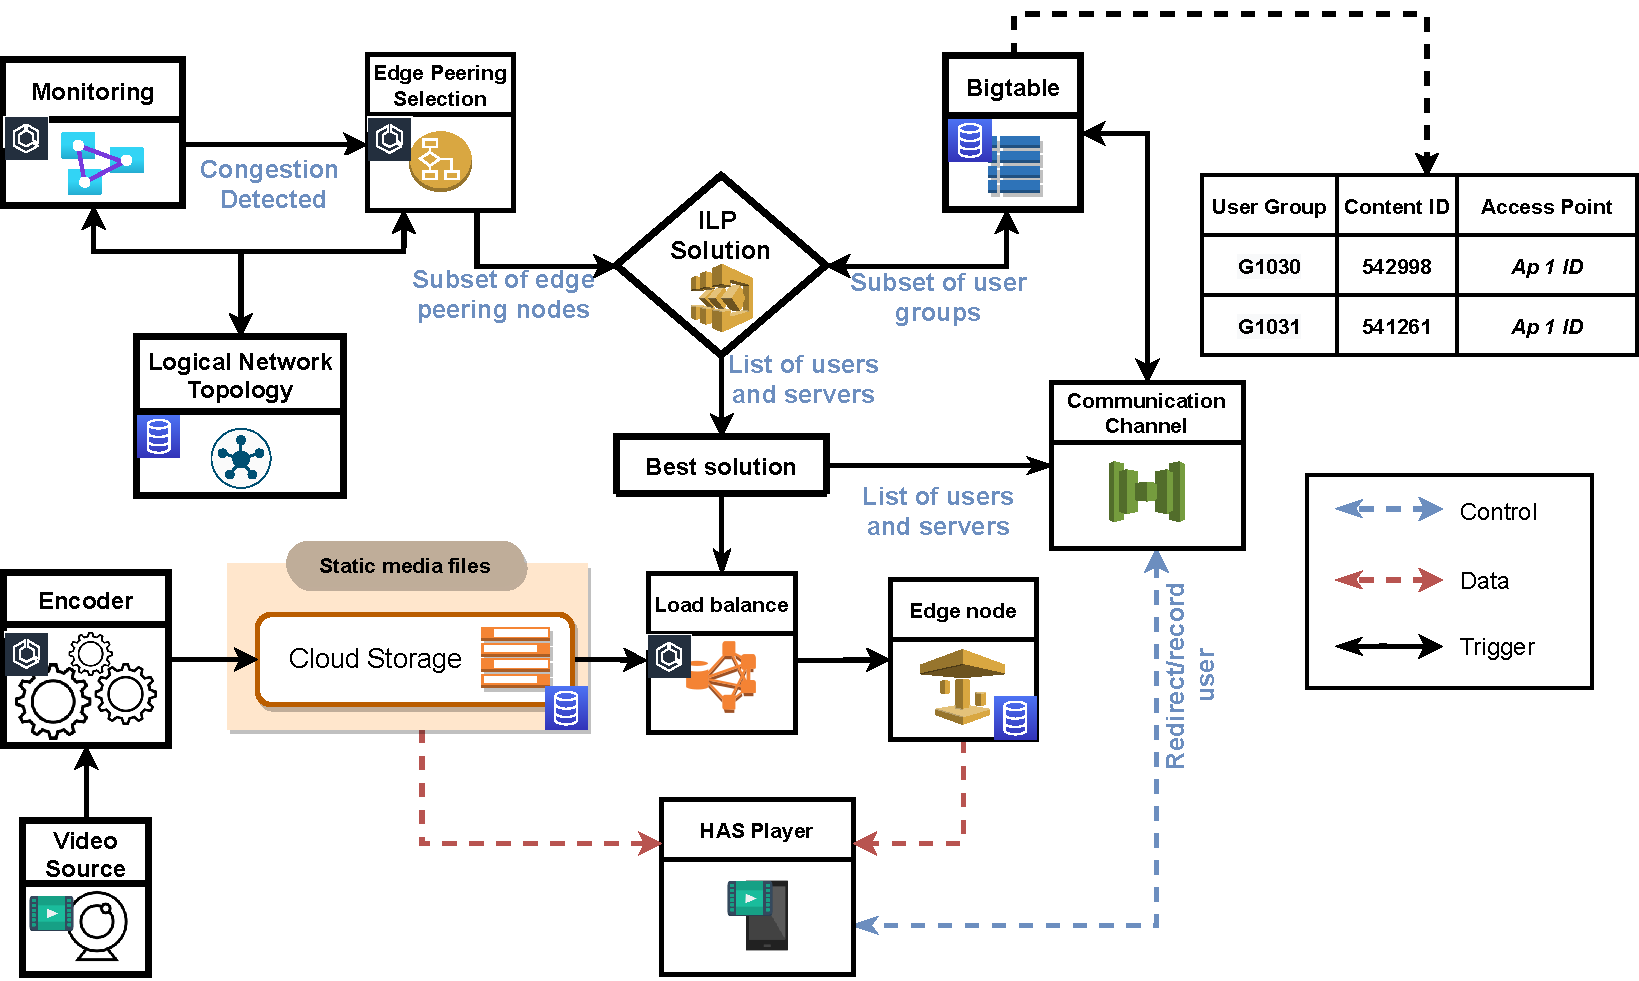
\includegraphics[width=\linewidth]{images/flow-model-infrastructure.pdf}
  \caption{Flowchart model of our proposed architecture.}
\end{figure}

Conforme ilustrado na Figura 2, apresentamos a arquitetura do sistema para realizar todas as solicitações/respostas necessárias ao serviço de streaming de vídeo. O cliente HAS primeiro solicita o manifesto ao servidor solicita o manifesto ao servidor HTTP. O reprodutor de traço solicita segmentos sequencialmente e adapta-se dinamicamente às condições da rede usando sua lógica de taxa de bits adaptável (ABR). Os esquemas ABR também levam em consideração o buffer de reprodução, recursos do dispositivo, preferências do visualizador e recursos de conteúdo. Enquanto o armazenamento em nuvem é essencialmente um servidor HTTP que armazena os pedaços de diferentes representações de vários conteúdos de vídeo e os arquivos de manifesto correspondentes. Além dos arquivos de manifesto regulares, o servidor HAS também armazena os arquivos de manifesto de qualidade para listar as qualidades perceptivas dos pedaços. Abaixo, discutimos os componentes em mais detalhes.


\subsubsection*{Componente de Comunicação}

O Canal de Comunicação funciona como canal controlador, no qual o componente é essencial para realizar a operação de comunicação com as redes celulares. A classe principal cria um canal de controle responsável por toda a comunicação entre as entidades. Neste trabalho são oferecidas duas funções de comunicação, \textit{i)} o redirecionamento após a execução do componente de otimização, desta forma são ativadas mensagens acionadas aos usuários que serão redirecionados para outro edge cache. Tal mensagem deve ser enviada após o servidor estar disponível para os usuários iniciarem uma conexão HTTP. Como segunda função oferecida, \textit{ii)} informações fornecidas pelos usuários, que incluem várias variáveis de entrada (por exemplo, largura de banda disponível, nível de congestionamento, QoE, nível de buffer, resolução do dispositivo, tipo de conteúdo).
%o ID do conteúdo solicitado e dados de estado do UE (por exemplo, ocupação de buffer).
As informações também podem auxiliar o módulo de otimização com relatórios periódicos sobre as BSs disponíveis e suas intensidades de sinal.


\subsubsection*{Componente de rastreamento}

O componente de rastreamento armazena o status do player em cada etapa e acompanha os players dos usuários. Antes de iniciar uma sessão de streaming, primeiro classifica em grupos os jogadores HAS com base em características específicas. Consideramos um conjunto de jogadores HAS $P = \{p_1,p_2, ..., p_N\}$, onde cada jogador $p_j \in P$ é colocado dentro de um grupo de usuários. Definimos os grupos de usuários como $G_{u,b_{i}}$ que contém um subconjunto de jogadores de usuários $p_j$ conectados com o mesmo BS $B(t) = \{b_{i}\}$ no momento $ t$ e solicita um conteúdo de vídeo específico $u$. Depois disso, cada conjunto de jogadores que pertencem ao mesmo grupo são agregados em um nó de peering de borda comum usando uma função de agregação simples (ou seja, conjunta).
Se o usuário iniciar com o pedido de manifesto a informação recebida contém o servidor atualizado, caso contrário, e o usuário já estiver visualizando o vídeo, um canal de comunicação realiza esta atualização. Ajudando assim a simplificar o processamento e a computação no componente otimizador.
% Em segundo lugar, ele formula o problema de seleção de representação como um Processo de Decisão Markov Parcialmente Observável (POMDP) com várias variáveis de entrada (por exemplo, largura de banda disponível, nível de congestionamento, QoE, nível de buffer, resolução do dispositivo, tipo de conteúdo, tipo de plano de assinatura), que representa nossa abstração do modelo POMDP consiste em três níveis, incluindo players, clusters e modelo POMDP de nível superior (agregação de todos os players). Por fim, em cada etapa, o módulo de recomendação de qualidade gerencia e armazena as decisões otimizadas por cluster resultantes do solver e, em seguida, passa essas saídas para o componente de comunicação.
Outro ponto importante é que o gerenciamento de players de usuários tende a se tornar mais fácil de manusear no lado do servidor, de modo que os usuários ativos são pré-organizados por este módulo.


\subsubsection*{Componente Monitoramento}
Para decidir quando um novo cache de peering de borda é necessário, o sistema também deve estar ciente das condições reais da rede. Portanto, um monitoramento de rede é necessário para realizar essa tarefa.
Basicamente, o componente de monitoramento tem a função de observar o uso da largura de banda do link da topologia da rede. Consideramos um conjunto de links com largura de banda $\Lambda$, onde cada link $\lambda_{\left \langle i,j \right \rangle} \in \Lambda$ está associado a um nó de origem $i$ e destino $j$ . A estimativa de largura de banda é baseada no pacote recebido/transmitido de cada interface de rede, a velocidade de download nos blocos recentes é robusta às flutuações de largura de banda. O objetivo do módulo de monitoramento é estimar periodicamente a taxa de transferência de cada rede de link. O módulo de monitoramento leva em consideração um determinado período $T$ e um estado de rede $\psi$.

Para estimar o throughput, o módulo de monitoramento calcula o número de pacotes recebidos durante cada período $T$. A taxa de transferência do link atual estimada é definida como $\lambda_{\left \langle i,j \right \rangle}(\psi, t)$. A largura de banda total no link de gargalo (fixo) é representada por $\lambda^{all}_{\left \langle i,j \right \rangle}(\psi, t)$. O uso estimado do link na próxima iteração $(t+T)$ e um novo estado de rede $\psi'$ são rotulados $\lambda_{\left \langle i,j \right \rangle}(\psi', t+ T) $. Aqui, em $\psi'$ estamos considerando mudanças físicas na rede como falha de link, assim como oscilações que ocorrem ao longo do tempo.% de tráfego cruzado, e assim por diante.
Finalmente, o módulo de monitoramento usa a taxa de transferência para estimar a taxa de transferência $\lambda_{\left \langle i,j \right \rangle}(\psi, t)$ ($\leqslant \lambda^{all}_{\left \langle i,j \right \rangle}(\psi, t)$)o sistema geral deve fornecer aos usuários.


\subsubsection*{Componente de Optimização}

O objetivo do componente otimizador é decidir sobre o número de servidores para minimizar a escala de infraestrutura necessária, mas também para maximizar a QoE dos usuários. Para isso, Esta seção apresenta um modelo de solução uma formalização em programação linear inteira (\textit{Integer Linear Programing} - ILP), uma classe coleta as entradas provenientes do monitoramento e, em seguida, recebe as entradas e procura maximizar o provisionamento de conteúdo de vídeo apresentado por redes multiníveis então, uma formalização da ILP recebe a entrada e busca maximizar o provisionamento de conteúdo de vídeo apresentado por redes multinível. 
Uma vez resolvido o problema de alocação, precisamos apenas considerar o problema de replicação dentro de cada edge cluster e seus grupos de usuários atribuídos (observe que a QoE dos grupos de usuários atribuídos é garantida com alocação estável). Em seguida, formulamos o problema de replicação de cluster único considerando um determinado cluster de borda F e os grupos de usuários atribuídos a F.

O objetivo do componente otimizador é decidir sobre o número de servidores para minimizar a escala de infraestrutura necessária, mas também maximizar o QoE dos usuários. Para isso, dividimos o tempo em duas classes principais, uma classe coleta as entradas provenientes do monitoramento, uma de programação linear inteira (ILP) recebe a entrada e busca maximizar o provisionamento de conteúdo de vídeo apresentado pelas redes multinível. % Na próxima seção, através de alguns experimentos, é possível verificar os impactos que ocorrem nos mecanismos de decisão ABR com uma topologia multinível simples.
%a provisão não apenas para atender a demanda de taxa de transferência de usuários finais em conteúdo de vídeo

A Tabela x.x resume os parâmetros e variáveis do modelo. Em relação aos parâmetros, o conjunto de pontos de entrada de onde são gerados os pedidos é rotulado como GW; estes correspondem aos gateways de onde os clientes acessam o ambiente Fog.


Como os clientes geralmente acessam os segmentos de vídeo de uma transmissão ao vivo sequencialmente, as demandas dos usuários para que os segmentos de vídeo sejam gerados na próxima janela de tempo curta podem ser estimadas aproximadamente pela audiência atual desse fluxo. Observe que as camadas superiores dentro da rede de borda tendem a atingir um grande número de usuários finais.
Para aumentar o número de atendimentos de um único nó, usamos a função $\chi(\psi, j)$. Onde $\lambda_{i}$ é o número de usuários no grupo $i$ e $p_{j}$ é a probabilidade de que o nó $j$ possa fornecer um streaming de vídeo para vários usuários.

\begin{equation}\label{cost_func}
\chi(\psi, j) = n(cP_{j}) * (1 - p_{j})
\end{equation}
\vspace{.05cm}

Para um servidor de borda arbitrário $j$, ele deve ter largura de banda suficiente para servir $A_j$. Assim, a seguinte restrição deve ser colocada:

\begin{equation}
x_{ij} * d_{i}( bt_{i}^{max}) \leq Bw_{p_{ij}^{k}} \\
\end{equation}
\vspace{.05cm}

onde $bi$ é a largura de banda consumida pelo visualizador $i$ e $B_j$ é a largura de banda total do servidor de borda $j$.

Seja $s_i$ uma transmissão ao vivo arbitrária de um canal ao vivo com uma determinada taxa de bits. Indicamos os segmentos de vídeo a serem gerados por $s_i$ em $T$ como $D^T_i$ (ou seja, $D^T_i = \{ v^{t_1}_i, v^{t_2}_i, ..., v ^{t_n}_i \}$, onde $(t_1,t_2,...,t_n)$ são os timestamps dos segmentos de vídeo ($v_1,v_2, ..., v_n$) gerados em $T$, respectivamente ). Se usarmos $L_{A_j}$ para denotar o conjunto não redundante de fluxos acessados por espectadores em $A_j$, a seguinte restrição na capacidade do cache deve ser colocada:

\begin{equation}
\sum^{n}_{i=1} x_{ij} \leq M_{j}y_{j}
\end{equation}
\vspace{.05cm}

onde $M(.)$ é a função que calcula o tamanho total do cache de um determinado conjunto de segmentos de vídeo, $c_j$ denota a capacidade de cache do servidor de borda $j$.

% Seleção de Caminho e Alocação de Recursos
Para suportar os serviços de vídeo demandados pelos usuários, um caminho ótimo definido para todos os fluxos de dados deve ser encontrado resolvendo o algoritmo proposto. Denote $P_{i}$ como um conjunto de caminhos incluindo todos os caminhos candidatos para o usuário $i$ e $P_{ij}$ como um subconjunto de $P_{i}$ incluindo todos os caminhos candidatos a partir do nó $j$. Um caminho $p_{ij}^{k} \in P_{i}$ significa o \textit{k-th} fluxo de caminho $i$ começando do nó $j$ e a taxa de dados correspondente deste caminho é denotada por $r_{ ij}^{k}$ se $p_{ij}^{k}$ estiver selecionado.

Assim, o problema proposto pode ser formulado da seguinte forma.

\begin{equation} 
\begin{aligned}
\min{} \quad &
\sum^{G_u}_{i=1}\sum^{F}_{j=1} c_{ij}x_{ij} + \sum^{F}_{j=1} f_{j} y_{j} \\
%
\text{Subject to} \quad & 
\sum^{F}_{j=1} x_{ij} = 1 \text{ } \forall i \in G_u \\
&
\sum^{n}_{i=1} x_{ij} \leq M_{j}y_{j} \\
&
x_{ij} * d_{i}( bt_{i}^{max}) \leq Bw_{p_{ij}^{k}} \\
&
x_{ij} \geq 0 \\
&
y_{j} \in \{0,1\} 
\end{aligned}
\end{equation}

Onde $F$ e $G_u$ são definidos como o conjunto de servidores de borda em um determinado cluster de borda e o conjunto de visualizadores atribuídos pela alocação estável de um para vários, respectivamente, e $x_{i,j}$ é definido do seguinte modo:

\begin{equation}\label{total_capacity_loss}
x_{i,j} =
\begin{cases}
1 & \text{if user } i \text{ requests to the server } j \\ 
0 & \text{otherwise }
\end{cases}
\end{equation}



% ==========================================

Na próxima seção, através de alguns experimentos, é possível verificar os impactos que ocorrem em mecanismos de decisão ABR com uma topologia multinível simples.
%a provisão não apenas para atender a demanda de taxa de transferência de usuários finais em conteúdo de vídeo

Uma vez que o componente de monitoramento detecta um link congestionado, o componente otimizador é acionado. Primeiramente, o módulo de seleção de peering de borda é responsável por reunir as entradas provenientes de monitoramento e bigtable, em que são um subconjunto da topologia da rede contendo os nós abaixo do link congestionado. Ao fazer isso, um subgrupo com os melhores usuários finais é selecionado dessa topologia de sub-rede.

Em seguida, utilizamos o conjunto de dados combinado para realizar uma solução no modelo ILP.
% Seleção de Caminho e Alocação de Recursos
Para suportar os serviços de vídeo demandados pelos usuários, um caminho ótimo definido para todos os fluxos de dados deve ser encontrado resolvendo o algoritmo proposto. Denote $P_{i}$ como um conjunto de caminhos incluindo todos os caminhos candidatos para o usuário $i$ e $P_{ij}$ como um subconjunto de $P_{i}$ incluindo todos os caminhos candidatos a partir do nó $j$. Um caminho $p_{ij}^{k} \in P_{i}$ significa o $k-th$ fluxo de caminho $i$ começando do nó $j$ e a taxa de dados correspondente deste caminho é denotada por $r_{ ij}^{k}$ se $p_{ij}^{k}$ for selecionado.

%\subsection{Solução de ILP proposta}


A estimativa da taxa de transferência usa a demanda que passa por $\widehat{s_{t+T}}$ para estimar a quantidade de taxa de transferência $D$ que o sistema geral deve fornecer aos usuários. Cada cliente tenta atingir uma qualidade alvo (maior taxa de bits de vídeo disponível) $Q$.
Além disso, introduzimos C, um coeficiente corretivo dinâmico para resolver os problemas de rede e servidor. Ele leva em consideração a taxa de bits média de vídeo $B (B \leqslant Q)$ exibida por todos os clientes que assistem ao fluxo e a taxa de falha $FR$, que é a parcela de clientes que não conseguiram obter a tempo a resposta de seu último pedido do servidor.

% As soluções de cache de conteúdo de requisições buscam minimizar o atraso médio de acesso ao conteúdo e maximizar a taxa média de requisições de conteúdo nos nós de edge cache, que nem sempre são alcançadas simultaneamente. Assim, um compromisso otimizado entre os dois objetivos é direcionado

% Curiosamente, a colocação de conteúdo e o agendamento de solicitações geralmente ocorrem em diferentes escalas de tempo: a popularidade do conteúdo geralmente varia lentamente, na escala de horas ou dias com base na medição e previsão de várias fontes; por outro lado, as decisões de agendamento de solicitações precisam se adaptar à dinâmica da localização do usuário e das condições do canal, que variam na ordem de segundos. Isso dificulta uma otimização conjunta para reagir prontamente às mudanças dinâmicas da rede; portanto, motiva a decomposição do problema geral em (i) o subproblema de gerenciamento de cache, que leva a popularidade do conteúdo a longo prazo como entrada, e (ii) o subproblema de escalonamento de solicitação de conteúdo, que leva em consideração as solicitações específicas recebidas, a condição de canal correspondente dos usuários e a disponibilidade de cache nas BSs e na CPU. Embora os dois subproblemas sejam tratados separadamente devido às suas diferentes escalas de tempo, o acoplamento entre os dois se reflete no fato de que a solução da política de colocação de cache é usada como entrada para a política de agendamento de requisições. Da mesma forma, a solução de agendamento de solicitações afetará a decisão de colocação de cache na próxima vez que for recalculada. Isso ocorre porque a popularidade do conteúdo é calculada com base no número de solicitações para cada conteúdo em diferentes BSs como resultado da política de agendamento de solicitações; portanto, após um longo período de escala de tempo (horas ou dias), a decisão de colocação do cache será feita com base na popularidade do conteúdo atualizado

% \subsection{Management Mechanism}

% Neste trabalho, o cliente e o servidor utilizam o protocolo HTTP na camada de aplicação para realizar todas as requisições/respostas necessárias. No lado do servidor, uma vez que um arquivo de mídia ~ (ou fluxo) esteja pronto, ele será preparado para streaming antes de ser publicado em um servidor HTTP padrão. O arquivo/stream original é particionado em segmentos~(também chamados \textit{chunks}) de tempo de reprodução equivalente, e várias versões (também chamadas de representações) de cada segmento são geradas que variam em taxa de bits/resolução/qualidade usando um codificador ou um transcodificador .
% Além disso, o servidor gera um arquivo de manifesto chamado descritor de apresentação de mídia~(MPD), que lista as representações disponíveis, incluindo informações como tempo de vídeo, disponibilidade de conteúdo, tipos de mídia~(ou seja, H.264 , H.265, etc. .), resoluções, larguras de banda mínimas e máximas, e a existência de várias alternativas codificadas de componentes multimídia, localização de segmentos de mídia na rede e outras características de conteúdo.

% No lado do cliente HAS, primeiro, o player de vídeo solicita o manifesto ao servidor HTTP e analisa as informações mencionadas acima. Dessa forma, ele pode começar a solicitar segmentos sequencialmente e adaptar-se dinamicamente às condições da rede usando sua lógica adaptativa de taxa de bits~(ABR). Os esquemas ABR também levam em consideração o buffer de reprodução, recursos do dispositivo, preferências do visualizador, bem como recursos de conteúdo, com pesos diferentes.
% Como a QoE do espectador precisa ser determinada em tempo real durante a reprodução, métricas objetivas são frequentemente usadas, incluindo o número de interrupções, duração do atraso de inicialização, frequência e número de oscilações de qualidade de vídeo. Por padrão, o HAS não requer nenhum esquema de adaptação específico, deixando os desenvolvedores de sistemas inovarem e implementarem seus próprios métodos.

% O controlador dentro do servidor CDN possui um canal de comunicação é criado com o usuário, assim as nossas mecanismos são capazes de se adaptar em tempo-real as necessidades da rede, bem como melhorar as

% \begin{algorithm} \caption{Mecanismo de gerenciamento multimídia em tempo real}
% \begin{algorithmic}[1]

% % \State Initilize $V(s) = 0$, for all $s \in \mathcal S^+$

% \State /* Phase 1: Make Decision related to the cache allocation and media content. */
% \State Initialize $a_i = 0$, for all viewer $i \in M$;
% \For {$i \in \textit{Grupos de usuários}$}
%     \State $j \leftarrow \textup{head of } S_{i}$;
%     \State Insert $i$ into $G_{j}$~($G_{j}^{k \cup i}$);
%     \If{$D(G_{j}^{0 \sim k}) \leq C_{j}$}
%         \State Label $G_{j}^{0 \sim k}$ with $j$;
%     \EndIf
%     % \State $v \gets V(s)$
%     % \State $V(s) \gets \sum_a \pi(s,a) \sum_{s'} \mathcal P_{ss'}^a [ \mathcal R_{ss'}^a + \gamma V(s')$
%     % \State $\Delta \gets \max(\Delta, |v- V(s)|)$
% \EndFor

% \State /* Phase 2: Redirecting viewers. */
% \For{viewer i with ai = 0}
%     \If{\textit{exists server} $j \in F$ \textit{with} $bd_j \geq b_i$ \textit{•}it{and} $s_i \in S_j$} 
%         \State $a_i \gets j$; $bd_j \gets (bd_j - b_i)$;
%     \EndIf 
% \EndFor

% \State /* Phase 3: Offload Media Content tasks. */

% \Ensure $S_i$
% \end{algorithmic}
% \end{algorithm}


\section{Experimental Setup}
\label{sec:experimental-setup}

\section{Modelagem e Análise de Hierarquias de Cache}
\label{sec:mechanism}

Consideramos hierarquias de cache dentro de uma rede de borda/nuvem representada como DAGs. As caches são substituições acionadas a cada cache que são ativadas para atender os usuários. Essa aproximação é baseada no rastreamento de um objeto atingido em um cache pai de volta a uma chegada correspondente.

A Figura 3 ilustra o cenário abordadoneste trabalho. Aqui, nós consideramos uma topologia em árvore binária com sete nós e um \textit{Cloud Provider} conectado ao nó raiz. Os últimos quatro nós são pontos de acesso~(AP) e os outros são pontos de peering de borda. Os nós AP são implementados em dispositivos sem fio que se comunicam via IEEE 802.11g em 2,4 GHz. Os APs têm conexões com fio para os pontos de peering de borda, enquanto os usuários finais também são sem fio. Cada usuário conectado ao AP está localizado a precisamente 8 metros de distância do AP. A largura de banda disponível é de 20Mbs nos links 0-1 e 0-2; e 30Mbs nos links 1-3, 1-4, 2-5 e 2-6.

\subsection{Abordagem de Decomposição}

O objetivo geral do nosso design é melhorar a QoE dos usuários de download de conteúdo, que se caracteriza principalmente pela latência do conteúdo e pela taxa de download. 
Apresentamos três estrategias que abordam os impactos identificados na Seção III na rede multicamada de borda/nuvem, ou seja, \textit{Only-Cloud}, \textit{QoS-Greedy} e \textit{ILP Solution}. 

O cenário \textit{Only-Cloud} usa apenas o nó Provedor de Nuvem para entregar o conteúdo de vídeo. Por outro lado, a abordagem \textit{QoS-Greedy} usa os nós da rede de borda, sempre que um congestionamento de link é detectado o \textit{QoS-Greedy} é ativado para escolher qual nó da borda para auxilar na entrega do vídeo.   A simulação começa com os usuários solicitando o vídeo da nuvem. Quando um link congestionado é detectado, o cache de borda abaixo do link é ativado. A partir daí, os usuários que recebem o vídeo pelo link congestionado são redirecionados para os nós de borda 1 e 2.


\subsection{Avaliação de QoE}

Dentre os modelos existentes na literatura, nós descrevemos como as metricas de QoE podem ser usadas para pontuar a satisfação do usuário. Primeiramente, cada pedaço de qualidade de vídeo é calculado por uma lei logarítmica sobre taxas de bits. A equação 1 mostra a transformação numérica da qualidade do video recebida pelo usuário. Cada vídeo tem $N$ segmentos e é codificado com $L$ níveis de taxa de bits. $r_i$ representa um nível de taxa de bits específico. A cada passo $i$, a qualidade do segmento $i$ é definida.

\begin{equation}\label{eq:equation-1}
q(r_i) = a_1 * log(a_2 * (r_i/ r_{L}))
\end{equation}
\vspace{0.1cm}

Para calcular a satisfação de cada usuário no longo prazo, é necessário um modelo flexível que inclua as métricas mais influentes para quantificar a QoE dos usuários. Consideramos a Equação 2 de [12], que consiste em quatro métricas: (a) a qualidade perceptual média do pedaço, (b) o número médio de oscilações de qualidade, (c) o número médio de eventos de estol e sua duração, e (d)) o atraso de inicialização. $K$ representa o total de segmentos do vídeo, $S_i$ é a duração da parada e $ST_i$ é o atraso de inicialização do usuário $i$.

\begin{equation}\label{eq:qoe-equation}
\begin{split}
QoE_i = \frac{1}{K} \sum_{k=1}^{K}q(r_{k}) - \frac{1}{K-1} \sum_{k=1}^{K-1}|q(r_{k+1}) - q(r_{k})| - \frac{1}{K}\sum_{k=1}^{K} S_{k} - ST_{i}
\end{split}
\end{equation}
\vspace{0.1cm}

O $QoE_{i}$ para cada usuário $i$ pode variar de 1 a 5, onde 1 = ruim, 2 = ruim, 3 = regular, 4 = bom e 5 = excelente.

\begin{figure}[htb!]
    \centering
    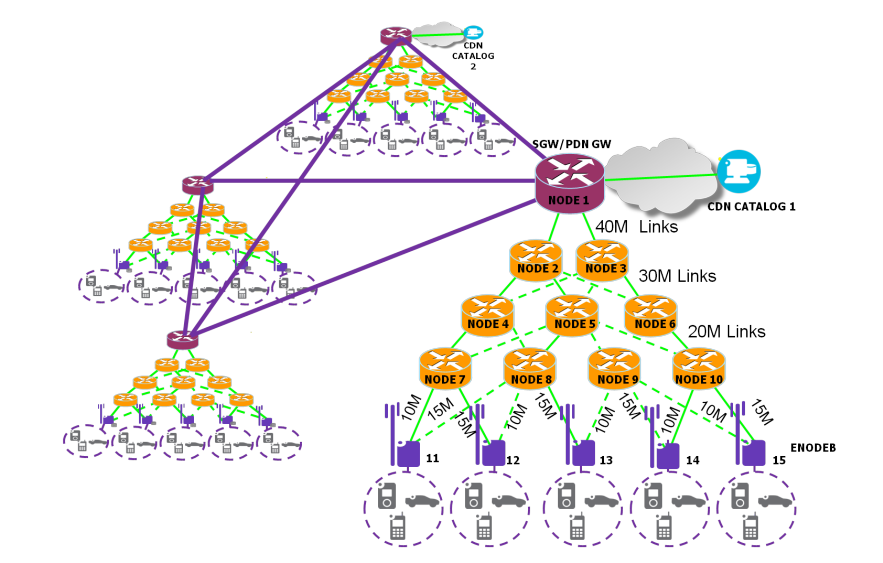
\includegraphics[width=\linewidth]{images/scenario.png}
    \caption{A General Overview of the multi-tier network environment.}
    \label{fig:multi-tier-network}
\end{figure}



\section{Resultados}
\label{sec:results}

\begin{figure*}
    %\vspace{-4em}
    \centering
    \subfigure[QoE]{
    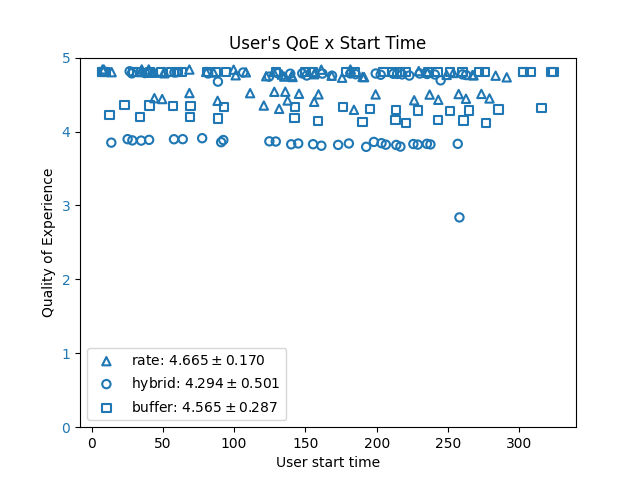
\includegraphics[width=0.32\linewidth]{charts/m_qoe_user.png}
    \label{fig:global-qoe-user}
    }
    \subfigure[HAS comparison]{
    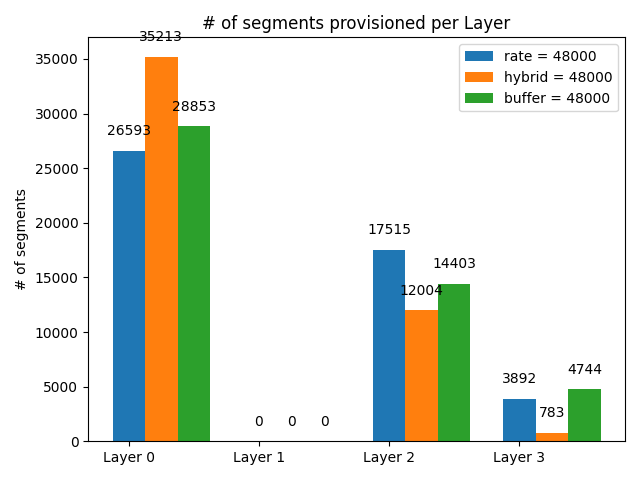
\includegraphics[width=0.3\linewidth]{charts/m_segments_per_layer_bu.png}
    \label{fig:plr-comparison-3}
    }
    \subfigure[Algorithm comparison]{
    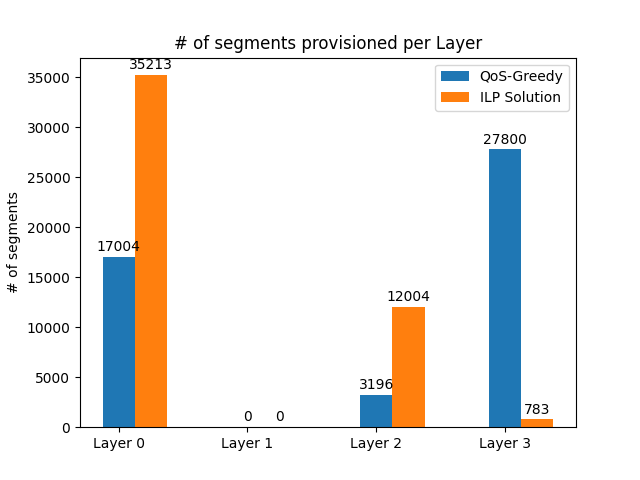
\includegraphics[width=0.32\linewidth]{charts/m_segments_per_layer_comp.png}
    \label{fig:plr-comparison-3}
    }
    \caption{Impact in a scenario (wall on the middle).
    }
    \label{fig:comparison-rof-3}
\end{figure*}


A Figura~\ref{fig:global-qoe-user} mostra o QoE global de cada usuário representada pode cada \textit{tick}, três algoritmos HAS são analisados com a solução ILP orquestrando a distribuição de video dentro da rede. Quando olhamos a media do desempenho sobre a perspectiva dos algoritmos HAS sendo executados pelo cliente, as heuristicas \textit{hydrid} e \textit{rate} tiveram um resultado melhor que o \textit{buffer}. O \textit{rate} teve uma leve oscilação entre os usuários, contudo os player sempre estiveram operando em boa qualidade, sem impactar diretamente o QoE e deixarem os usuários cairem no \textit{score}.

%Quando paramos para analisar a distribuição de requisições entre os níveis. 

Os experimentos ilustrados nas Figuras 4, 5 e 6 mostram a QoE média calculada pela Equação 2 quando há 15, 20 e 25 usuários por ponto de acesso solicitando vídeos na infraestrutura simulada. Cada boxplot representa os cenários somente nuvem, cache de borda e mobilidade. O desempenho médio geral do cache de borda é melhor do que os cenários somente nuvem e mobilidade, principalmente devido às escolhas de nós nos nós de peering de borda para atender às solicitações dos usuários. Por exemplo, no experimento Edge cache, quando ocorre congestionamento em links intermediários e 0,1 e e 0,2 , os nós de peering de borda são ativados para atender os usuários finais abaixo desses nós. Dessa forma, o tráfego que passa pelo link ascendente agora será suavizado, para que os usuários possam ter sua QoE aprimorada a um nível excelente. Como os usuários solicitam segmentos dos nós mais próximos e sem enlace de congestionamento em cenários com Edge cache, como esperado, observamos um aumento de QoE. A diferença de desempenho dos cenários somente na nuvem e de mobilidade para o experimento de cache de borda está próxima de um nível de satisfação para 15 e 20 usuários e aproximadamente dois níveis de satisfação para 25 usuários

Uma discussão interessante ocorre quando a QoE por usuário é analisada separadamente. De acordo com os resultados numéricos, a QoE final tende a piorar à medida que o número de usuários ativos aumenta. No entanto, isso não é totalmente verdade para o cenário de cache de borda, em que o QoE final para cada usuário permanece próximo. O desvio padrão de 0,037, 0,162 e 0,273, respectivamente, para cenários com 15, 20 e 25 usuários por AP, indica uma QoE mais próxima entre os usuários. Apenas no cenário de 25 usuários por AP, a QoE média apresentou queda com satisfação próxima da regular. Em contraste com os outros dois cenários apresentando uma satisfação dos usuários de boa a excelente. Enquanto para cenários de mobilidade e somente nuvem, a rede opera com um alto desvio padrão. À medida que o número de usuários aumenta, alguns outliers começam a aparecer com o pior nível de satisfação, ficando entre ruim e inadequado.

Com base nessas observações, uma estratégia simples de mover o vídeo para a borda pode melhorar significativamente a QoE do usuário. Desta forma, o sistema de transmissão de vídeo pode proporcionar qualidades de satisfação ao usuário e mantê-lo assistindo o vídeo até o final. No entanto, se não houver um gerenciamento correto das conexões em tempo real e um mecanismo dinâmico para lidar com uma carga variável proveniente, por exemplo, da mobilidade dos usuários, podemos concluir que o impacto introduzido pelas alterações do AP pode diminuir significativamente sua QoE. A experiência do usuário pode acabar piorando mesmo usando a borda da rede. O gerenciamento adequado de conteúdo multimídia pode ser feito no qual o VoD se concentra em fornecer uma melhor QoE para as mudanças de conexão dos usuários. Um mecanismo de migração de conteúdo na borda e nas camadas superiores pode atenuar o problema. Além disso, realizar um reencaminhamento entre as conexões dos usuários ativos e os nós do servidor pode ajudar a melhorar e equilibrar a QoE do usuário.

\section{Conclusion}
\label{sec:conclusion}

Conclusions may be used to restate your hypothesis or research question, restate your major findings, explain the relevance and the added value of your work, highlight any limitations of your study, describe future directions for research and recommendations. 

In some disciplines use of Discussion or 'Conclusion' is interchangeable. It is not mandatory to use both. Please refer to Journal-level guidance for any specific requirements. 



\bibliographystyle{sbc}
\bibliography{sbc-template}

\end{document}
